\section{Open Discussion and scalability}
\label{sec:discussion}
Our approach is about modeling, design, and implementation of software architecture, especially monolithic architectures.
In this section we describe the differences between our approach and architecture description languages \cite{medvidovic2000classification}, which provide precise and formal notations for describing architectures.
We also discuss how our approach can be applied to distributed architectures, to ALF, and the main limitation of our approach in applying to synchronize architecture models with different programming languages.  

%1. compare with ADLs, why use UML elements such as ports, connectors, state machines
\noindent
\tb{Architecture description language}:
The idea of our approach is to have architectural information right at the code level by proposing additional ad-hoc programming constructs.% for architectural modeling elements.
At a first glance, the code written with these additional constructs looks like the code in ADLs.
However, our approach and the ADLs are fundamentally different.
The ADLs are often used for architecture description, analysis, and verification \cite{robbins1998integrating}. 
The Smalltalk-based SCL component language \cite{fabresse2006scl} is even operational.
However, its acceptance does not gain as much as mainstream object-oriented languages.
Our additional constructs remain the extended language as an object-oriented programming language dedicated for system development including debugging and execution.
The code written in ADLs can be translated into programming language code. 
But, the development activities such as compilation, debugging, and execution of this translated code is completely separated from the ADLs code.
Our approach, on the other hand, allows the use of architectural information elements directly at the code level for these development activities. 
Furthermore, the additional constructs in our approach are often used by programmers while the ADLs by architecture analysts.
%Our approach is more likely embedding an architectural language as 
%Many architecture description languages (ADLs) have been proposed 

\begin{comment}
\noindent
\tb{Architecture constraints reasoning}:
%addition: how to give contract/constranit information for architecture reasoning
One might ask whether the synchronization can be applied in case model elements contain architectural constraints such as timing constraints as seen with ADLs for architecture reasoning.
As previously described, our approach can synchronize functional constraints such that a port with required interface must be connected to a port providing the same interface.
In future, we plan to add more attributes to our port constructs for representing non-functional constraints to reason about contracts between required and provided ports.
\end{comment}

\noindent
\tb{Distributed architecture}:
%2. How to deal with distributed architectures? ==> using connectos + interaction components + more information in the bindings refer to zeromq paper
A question to our approach is whether it can be used for development of distributed architectures such as client-server architecture.
Currently, it is only applied to a monolithic architecture.
However, we believe that we can apply the approach to distributed architectures with some extensions.
In our previous work \cite{Pham2014}, we propose to use \ti{interaction components} to model the communication between components within a distributed system.
For a client-server system model as in Fig. \ref{fig:clientserverpapyrus} (a) in which the client requests services from the server through a remote interface \ti{IPush}.
The connector between the components ports is transformed into an \ti{ic} interaction component typed by \ti{AsyncCall} as in Fig. \ref{fig:clientserverpapyrus} (b).
The \ti{AsyncCall} interaction component is modeled as UML components/classes and then translated to middleware-based interaction implementation such as ZeroMQ (see \cite{Pham2014} for more details).
In the generated extended code in Fig. \ref{fig:clientserverpapyrus}, the system at the client-side contains the client, the \ti{ic} interaction component, and a binding from the \ti{p} required port of the client to the \ti{q} provided port of \ti{ic}.
The system at the server-side, on the other hand, consists of \ti{server}, \ti{ic}, and a binding from the \ti{q} provided port of \ti{server} and the \ti{p} required port of \ti{ic}.
\ti{AsyncCall} realizes the communication implementation between the two sides.
For example, for each call from the client through its port, \ti{AsyncCall} establishes a socket connection, marshals and send the call's parameters to the \ti{ic} interaction component at the server-side.
This latter indeed demarshals the received data to extract the parameters values sent by the client, and calls the corresponding method of the server via the \ti{p} port of \ti{ic}.  

The propagation of modifications in the model and the code is as followings:
\begin{itemize}
	\itemsep0cm
	\item If the model is modified:
		\begin{itemize}[\footnotesize]
			\itemsep0cm
			\item If the client is modified, propagate the modifications to the client-side code.
			
			\item If the server is modified, propagate the modifications to the server-side code.
			
			\item If the interaction component is modified, propagate the modifications to the interaction component code at both of the sides.
		\end{itemize}	
	
	\item If the code is modified:
		\begin{itemize}[\footnotesize]
			\itemsep0cm
			\item If the client at the client-side is modified, propagate the modifications to the client component at the model level.
			
			\item If the server at the server-side is modified, propagate the modifications to the server component at the model level.
			
			\item If the interaction component is modified at the either side, propagate the modifications to the interaction component at the model level.
		\end{itemize}
\end{itemize} 
 


\begin{figure}
	\centering
	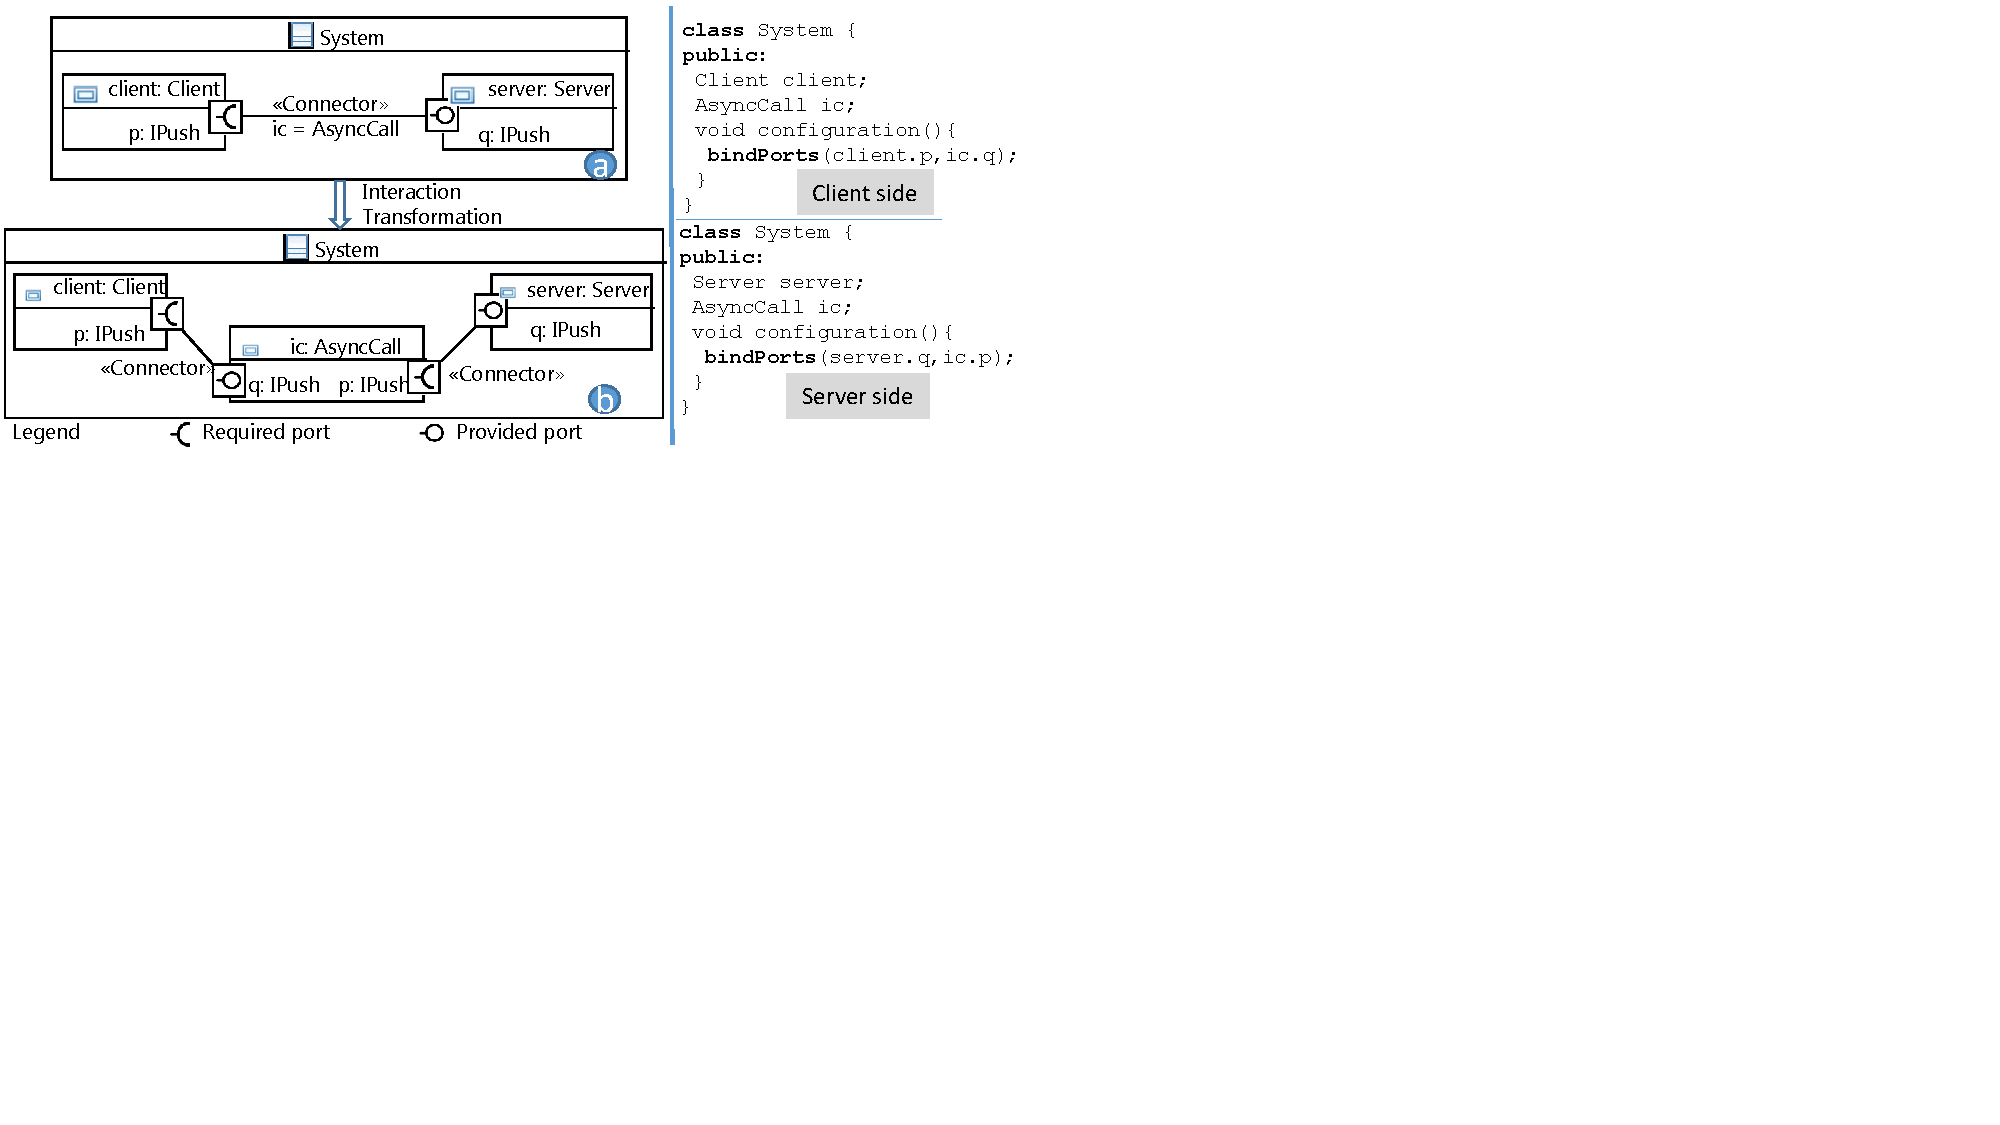
\includegraphics[clip, trim=0cm 11.4cm 16.8cm 0.2cm, width=\columnwidth]{figures/clientserverpapyrus.pdf}
	\caption{Client-server example including interaction component transformation, client-side, and server-side code} 
	\label{fig:clientserverpapyrus}
\end{figure}

\noindent
\tb{Action Language for Foundational UML (ALF):}
Back to the introduction section, we mentions the use of ALF as a fine-grained behavioral expression language for operation bodies to preserve modeling consistency and enable a full model-centric approach, and full-fledged code generation for embedded systems \cite{ciccozzi2015generation}.
The main limitation that makes this approach not sound is that ALF is not common, even unknown in the programming community with very strong and widely used programming languages such as Java and C+. 
We believe that a harmonization of using ALF and common programming languages would benefit advantages of both of the modeling and programming community.
Therefore, a further step, that builds upon our approach and synchronizes ALF-based fine-grained behaviors with programming code, should be included in future work.
This extension might be based on the mapping between ALF and C++ proposed in \cite{Ciccozzi2016}. 

\noindent
\tb{Language support limitation}:
%3. Limitations: ad-hoc constructs are built based on built-in language features ==> the approach is hardly applied to many languages but C++, Java
Our approach is based on using built-in programming language features to add new programming constructs to the language.
Therefore, it is dependent on the programming language that we want to synchronize with UML. 
It is currently applicable to C++ with macros, Java and C\# with annotations, and Python with macropy \cite{macropy}.
More languages should be investigated to elaborate the approach.%and cannot be applied to all programming languages.

 


